\section{Setup Environment}

We simulate all path finding processes based on the framework of 
GridWorld\cite{web:gridworld}, an AP case study project from collegeboard
\footnote{https://www.collegeboard.org/}. It provides graphical user interface 
based on Java AWT where visual objects can interact and perform customized 
actions in a two-dimensional grid map. In the next part, we will first illustrate
original GridWorld framework and our enhancement of displaying colored path.
This mainly involves the engineering work, so if you want to directly delve 
into algorithm analysis, please skip it.

\subsection{GridWorld Architecture and Modification}

The source code of original GridWorld project is placed in $src/main/framework$
folder and its structure can be divided into four parts, as shown in Figure 
\ref{fig:framework-structure}.

\begin{figure}[ht]
  \centering
  \begin{subfigure}[b]{0.45\textwidth}
    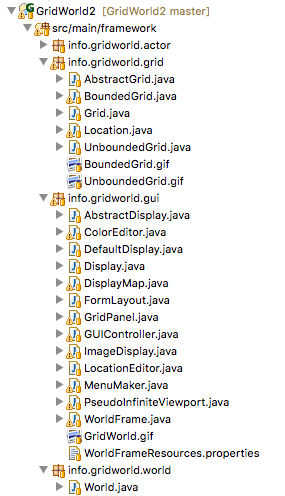
\includegraphics[width=0.9\textwidth]{framework-structure}
    \caption{GridWorld structure}
    \label{fig:framework-structure}
  \end{subfigure}
  ~
  \begin{subfigure}[b]{0.45\textwidth}
    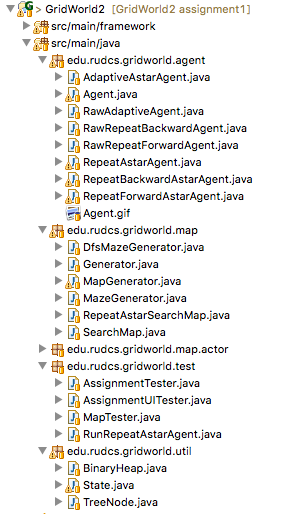
\includegraphics[width=0.9\textwidth]{project-structure}
    \caption{Project structure}
    \label{fig:project-structure}
  \end{subfigure}
\caption{Structure of GridWorld framework and path-finding project}
\end{figure}

The $actor$ package contains objects whose behavior on the map can be arbitrarily 
defined by rewriting $act$ method in each inherited class:

\begin{lstlisting}
%%@Override%%
public void act()
\end{lstlisting}

The $grid$ package defines features on bounded and unbounded grid map as well 
as connections between map and actors. The $gui$ package encapsulates low-level
Java AWT to provide APIs for visualization and interactions of map and actors.
The $world$ package provides high-level integration of actors and world.

In order to visualize the presumed unblocked path and the set of nodes expanded
and explored after each planning, we enhance the $GridPanel$ class in the 
GUI package by implementing the method below:

\begin{lstlisting}
private void drawColoredLocations(Graphics2D g2)
\end{lstlisting}

Meanwhile, following five abstract methods related to colored grid are added 
to $Grid$ interface and classes like $BoundedGrid$ and $UnboundedGrid$ are 
responsible to implement color configuration on each grid.

\begin{lstlisting}
ArrayList<Location> getColoredLocations();
Color getColor(Location loc);
void putColor(Location loc, Color color);
void removeColor(Location loc);
void resetColors();
\end{lstlisting}

The source code related to assignment is placed in $src/main/java$ folder, as 
shown in Figure \ref{fig:project-structure}, which are divided into five packages.
The $agent$ package defines the simulated agents equipped with specific navigation 
algorithm for solving goal-directed path-finding problem. The $map$ package 
provides APIs for generation of random map and corridor-like maze. The $map.actor$ 
package defines some static object on the map like obstacles and goal. The $test$
package contains simulation program for experiment and testing. The $util$
package includes some self-defined data structures to be used in storing 
intermediate result of algorithm.

\subsection{How to Run}

Our project is built and packed by Gradle\footnote{http://gradle.org/}, 
an open-source build automation tool. First, you should install and setup Gradle
environment on your computer, and install Gradle plugin for Eclipse, named 
"Gradle Integration for Eclipse". Then, download complete source code of the 
project, which is attached in Sakai or available on the 
Github\footnote{https://github.com/orcax/GridWorld2}. Finally, inside Eclipse,
click $File\rightarrow Import\rightarrow Gradle\rightarrow Gradle~Project$ to
import project. All runnable programs are placed in $test$ package.

\subsection{Maze Generation Algorithm}

In the experiment, we mainly use two kinds of grid map, namely random map with 
discrete obstacles and random maze with consecutive obstacles.
